%Summary here
The system evaluation complements the system implementation by measuring the performance of the developed solution, answering RQ2. This evaluation process will be carried out following a sequential approach.

This section details the method and the principles that will be used to carry out the system evaluation process, measuring the performance (throughput, measured in rows/second) of reading and writing on Delta Lake or Apache Hudi while on \gls{HopsFS} of Spark-based and Rust-based pipelines. 

\subsection{Evaluation Process and Research Paradigm}
\label{subsec:eval_process_and_research_paradigm}

The research process will follow a sequential approach described in Figure \ref{fig:DevProcessRQ2}. Each step of this process is related to one of the goals (G5-G8) associated with the RQ2 in Section \ref{sec:goals}.
The relationship between each activity and the associated goal(s) is here explained:
\begin{enumerate}
    \item \textbf{Design experiments}: this activity maps perfectly to G5, designing the experiments that will be conducted to evaluate the performance difference in performance between Spark-based access to Apache Hudi compared a the delta-rs \cite{DeltaioDeltars2024} library-based access to Delta Lake, in \gls{HopsFS}. 
    \item \textbf{Perform experiments}: this activity maps perfectly to G6, using the code implementation (D1) to conduct the designed experiments on the analyzed systems.
    \item \textbf{Transform data according to metrics}: this activity is necessary to fulfill G7, as data visualization requires data to be properly formatted. In this activity data is modified, performing a division between the size of the table inputted and the read or write time. This allows data to be in the wanted metric i.e. rows/second.
    \item \textbf{Visualise results}: this activity maps perfectly to G7, visualizing the experiments' result according to the selected metric, i.e. throughput measured in rows/second. This activity also generates a deliverable (D2) composed of the experiments results complete with tables and histograms, i.e. Section \ref{}.
    \item \textbf{Analyse results}: this activity maps perfectly to G8, analysing and interpreting the results delivered in D2. This contributes to D3, generating the analysis of results, i.e. Section \ref{}.
\end{enumerate}
\begin{figure}[!ht]
    \begin{center}
      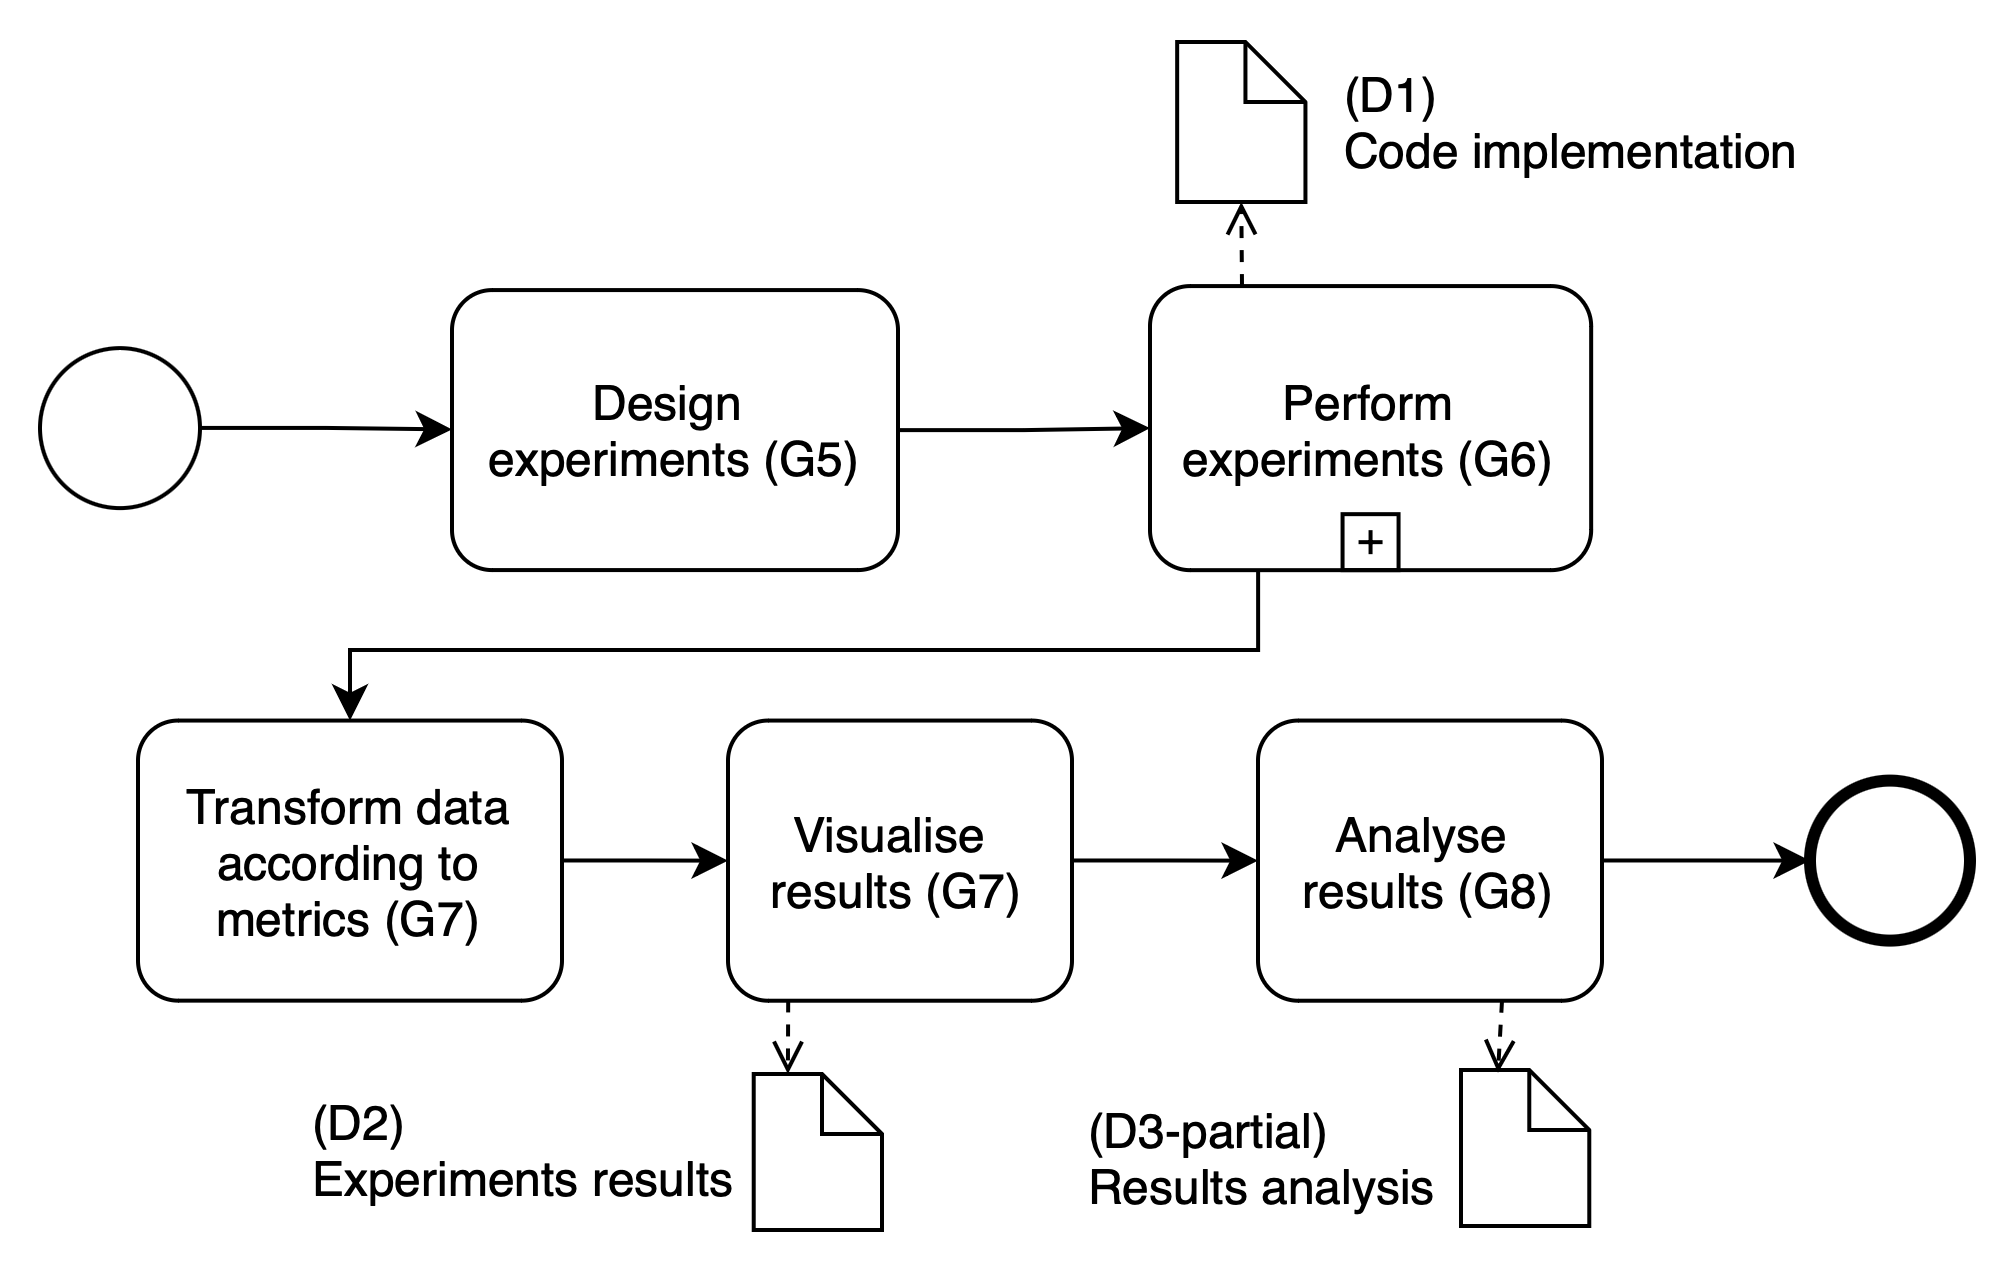
\includegraphics[width=\textwidth]{figures/3-method/research_process_rq2.png}
    \caption{\gls{BPMN} diagram of the System evaluation process answering to RQ2. Each activity is associated with a specific Goal (\gls{G}). The process produces two deliverables (\gls{D}), the experiments results (D2) and a results analysis (D3-partial).}
    \label{fig:DevProcessRQ2}
    \end{center}
\end{figure}

The research paradigm consists of a quantitative analysis based on repeated runs on the implemented system. The results of the benchmarks are then analyzed performing a visual comparative approach.

\subsection{Dataset}
\label{subsec:dataset}

The data that will be used to perform the read and write operations comes from \glsentryshort{TPC}-H benchmark suite\cite{TPCHHomepage}. \glsentryshort{TPC}-H is a decision support benchmark by \gls{TPC}. It consists of a series of business-oriented ad-hoc queries designed to be industry-relevant \cite{transactionprocessingperformancecounciltpcTPCH_v301pdf1993}. The data coming from this benchmark suite was used as
it provides a recognized standard for data storage systems \cite{TPC_benchmarks_2000}, and it has already been used in similar related work \cite{raasveldtDuckDBEmbeddableAnalytical2019, behmPhotonFastQuery2022}. Any part of the data can be generated using the TPC-H data generation tool \cite{TPCCurrentSpecs}.

The \glsentryshort{TPC}-H benchmark contains eight tables, of these two, SUPPLIER and LINEITEM, were selected for the following reasons. The two tables are respectively the smallest (10000 rows) and largest (6000000 rows) tables whose size (number of rows) depends on the \gls{SF}. The \gls{SF} can be varied to obtain tables of different sizes (number of rows), allowing a progressive change in the table size (number of rows). 

The SUPPLIER table has seven columns, while the LINEITEM table has sixteen. This influences the average size of memory each row occupies. This means the metric selected (throughput, measured in rows/second) cannot be used to compare results across different tables. This is the reason why the comparative evaluation only considers different configurations on the same table. 

For this project, five table variations were used to benchmark the code solution as D1. \gls{SF} was varied to obtain a table at each significant figure, from 10000 rows to 60000000 rows. These are the tables:
\begin{enumerate}
    \item \textit{supplier\_sf1}: size = 10000 rows
    \item \textit{supplier\_sf10}: size = 100000 rows
    \item \textit{supplier\_sf100}: size = 1000000 rows
    \item \textit{lineitem\_sf1}: size = 60000000 rows
    \item \textit{lineitem\_sf10}: size = 60000000 rows
\end{enumerate}

\subsection{Experimental Design}
\labe{subsec:experimental_design}
% Description of which benchmarks will be performed and how. Here it needs to be explained the environment where the benchmarks will be run (Snurran), which tests are run and why in this particular way.
%
% Talk about the selection of the questions: How do the performances vary if: (1) the new implemented pipeline is used vs. the old pipeline. (2) a simple localFilesystem implementation is used vs. writing on \gls{HopsFS} (3) varying the CPU configuration (4) we have different table sizes. 

The experiments aim to highlight the differences between the newly implemented system based on the delta-rs library, and the legacy Spark-based system. To isolate the benefit of using delta-rs over Spark and provide a baseline, three different testing pipelines were designed:
\begin{enumerate}
    \item \textbf{delta-rs - \glsentryshort{HopsFS}}: the system implemented in Chapter \ref{ch:implementation}. It comprises a Rust pipeline with Python bindings, enabling performing operations (i.e., reading, writing) on Delta Lake tables. This pipeline writes on \gls{HopsFS}.
    \item \textbf{delta-rs - \glsentryshort{LocalFS}}: this pipeline uses the same library as the system implemented, but saves data on the \gls{LocalFS}. This provides a comparison within the delta-rs library, isolating the impact on performance caused by writing on \gls{HopsFS}, a distributed file system.
    \item \textbf{Legacy Spark pipeline}: this pipeline uses the Hopsworks Feature Store to write data on Hudi tables. This system makes use of a pipeline based on Kafka, and Spark to write data on the Hudi tables, saved on \gls{HopsFS}. 
\end{enumerate}

Furthermore, the experiments will verify how the performances of the three systems will change based on the \gls{CPU} resources provided (namely 1 core, 2 cores, 4 cores, 8 cores). Each time the testing environment will be modified accordingly, creating a new \gls{VM} where the experiments will run with increasingly more resources. These \gls{CPU} configurations were chosen together with the industrial supervisor, according to the typical Hopsworks use case.

The data used for experiments, as described in Section \ref{subsec:dataset}, will come from two different tables. These are modified according to a \gls{SF}, for a total of five times.

In conclusion, the experiments conducted will be a total of 3 (pipelines) times 4 (\gls{CPU} configurations) times 5 (tables) times 2 (read and write operations), i.e. 120 experiments, performed 50 times each to create statistically significant results.

\subsection{Experimental environment}
% Describe Snurran

The experimental environment consists of a physical machine in Hopsworks' offices, virtualized enabling remote shared development. The \gls{CPU} details of the machine are present in Listing \ref{lst:cpu_snurran}, noting that only eight cores at maximum were accessed during the experiments.

The machine mounts about 5.4 TBs of \gls{SSD} memory. This allows the machine to have fast read and write speed, 2.7 GB/s, and 1.9 GB/s respectively (measured with a simple \textit{dd} bash command). 

The experimental environment will be set up with a Jupyter Server of different CPU cores, depending on the experiment (1 core, 2 cores, 4 cores or 8 cores). The Jupyter server is allocated by default with 2048 MB of \gls{RAM}, out of the .. available on the experimental machine. This amount will be adjusted during the experiments according to the needs of the experiments, 

\begin{lstlisting}[language=bash, caption={Output of a \textit{lscpu} bash command on the test environment.}, label={lst:cpu_snurran}, frame=tb]
Architecture:            x86_64
  CPU op-mode(s):        32-bit, 64-bit
  Address sizes:         48 bits physical, 
                         48 bits virtual
  Byte Order:            Little Endian
CPU(s):                  32
  On-line CPU(s) list:   0-31
Vendor ID:               AuthenticAMD
  Model name:            AMD Ryzen Threadripper 
                         PRO 5955WX 16-Cores
    CPU family:          25
    Model:               8
    Thread(s) per core:  2
    Core(s) per socket:  16
    Socket(s):           1
    Stepping:            2
    Frequency boost:     enabled
    CPU max MHz:         7031.2500
    CPU min MHz:         1800.0000
    BogoMIPS:            7985.56
Virtualization features: 
  Virtualization:        AMD-V
Caches (sum of all):     
  L1d:                   512 KiB (16 instances)
  L1i:                   512 KiB (16 instances)
  L2:                    8 MiB (16 instances)
  L3:                    64 MiB (2 instances)
\end{lstlisting}
\FloatBarrier

\subsection{Evaluation Framework}
% Describe which metrics are used to evaluate the system. Which metrics were used during the experiments
%
% What I would like to say is essentially that:
% This evaluation section objective is to: Verify The system requirements defined in ... , and compare the performance (defined as throughput in RQ2) with older systems. Explain how both of these things are done

The system evaluation framework is designed to evaluate three key aspects of the system:
\begin{enumerate}
    \item \textbf{Functional requirements}: defined in Section \ref{subsec:requirements}, functional requirements will measured by verifying the success or failure of running an experiment. By design, this will not happen, as the system implementation phase, continues until all functional requirements are met.
    \item \textbf{Non-functional requirements}: defined in Section \ref{subsec:requirements}, non-functional requirements are: consistency, maintainability and scalability. The first two requirements are mainly addressed during implementation, while scalability is measured during the system evaluation experiments. The metric used for measuring this requirement is the throughput measured in rows/second as defined in RQ2.
    \item \textbf{How does the system compare to other pipelines?}: this question answers directly RQ2, measuring the throughput (rows/second) of the different pipelines, defined in Section \ref{subsec:experimental_design}. Results are then compared with a visual approach a.
\end{enumerate} 


RQ2 clearly defines throughput as the evaluation metric for measuring the performance between the two analysed systems. Section \ref{subsec:eval_process_and_research_paradigm} states that the approach performed in the system evaluation will be comparative, comparing different pipelines using the same data with the same computing resources.

The Requirements defined in Section \ref{subsec:requirements} 


on the success of the experiment, i.e. completing the read or write of the inputted data (



\subsection{Assessing Reliability and Validity}
% Here explain how the readability and validity of the collected data was addressed. Mainly here the bootstrapping method need to be explained and how it achieves getting a CI without making assumption on the data distribution

Results are significant according to their reliability and validity. In this project work, to ensure the reliability of the experiments results on the system performance, each experiment will be performed fifty times. This number was agreed as a balance between consistency and the limited resources available (in terms of time and computing resources).

Probably due to the complex nature of the pipeline tested, the data distribution of results could vary from one experiment to the other. This hampers the possibility of comparing results, greatly impacting the relevance of the results analysis. To restore the validity of the data collected a bootstrapping technique will be used. Data will be resampled with substitution a thousand times, then an average with a confidence interval for each experiment will be calculated. This will benefit the accuracy of the results presented.